% Created by tikzDevice version 0.8.1 on 2015-06-29 01:14:31
% !TEX encoding = UTF-8 Unicode
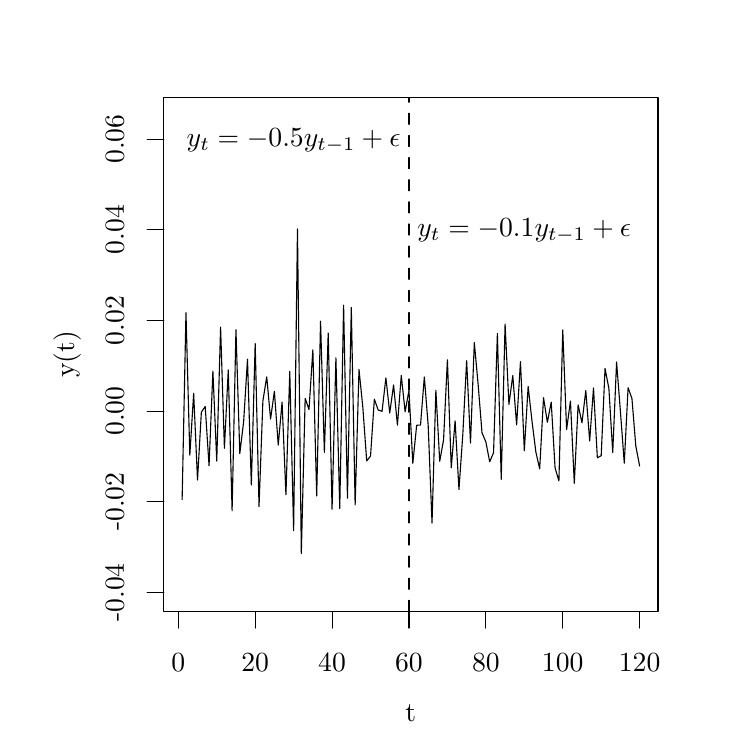
\begin{tikzpicture}[x=1pt,y=1pt]
\definecolor{fillColor}{RGB}{255,255,255}
\path[use as bounding box,fill=fillColor,fill opacity=0.00] (0,0) rectangle (252.94,252.94);
\begin{scope}
\path[clip] ( 49.20, 42.00) rectangle (227.75,227.75);
\definecolor{drawColor}{RGB}{0,0,0}

\path[draw=drawColor,line width= 0.4pt,line join=round,line cap=round] ( 55.81, 82.35) --
	( 57.20,149.96) --
	( 58.59, 98.44) --
	( 59.98,120.83) --
	( 61.37, 89.46) --
	( 62.76,114.00) --
	( 64.15,116.06) --
	( 65.54, 94.64) --
	( 66.93,128.85) --
	( 68.32, 96.29) --
	( 69.71,144.75) --
	( 71.09,100.94) --
	( 72.48,129.24) --
	( 73.87, 78.39) --
	( 75.26,143.81) --
	( 76.65, 99.06) --
	( 78.04,110.56) --
	( 79.43,133.12) --
	( 80.82, 87.65) --
	( 82.21,138.82) --
	( 83.60, 79.89) --
	( 84.99,118.00) --
	( 86.38,126.76) --
	( 87.77,111.52) --
	( 89.15,121.56) --
	( 90.54,102.08) --
	( 91.93,117.62) --
	( 93.32, 84.17) --
	( 94.71,128.75) --
	( 96.10, 71.21) --
	( 97.49,180.19) --
	( 98.88, 62.89) --
	(100.27,119.01) --
	(101.66,114.94) --
	(103.05,136.56) --
	(104.44, 83.72) --
	(105.83,146.88) --
	(107.21, 99.43) --
	(108.60,142.59) --
	(109.99, 78.91) --
	(111.38,133.65) --
	(112.77, 79.20) --
	(114.16,152.66) --
	(115.55, 82.90) --
	(116.94,151.86) --
	(118.33, 80.48) --
	(119.72,129.45) --
	(121.11,115.73) --
	(122.50, 96.38) --
	(123.89, 98.13) --
	(125.27,118.68) --
	(126.66,114.78) --
	(128.05,114.30) --
	(129.44,126.40) --
	(130.83,113.70) --
	(132.22,123.84) --
	(133.61,109.32) --
	(135.00,127.25) --
	(136.39,114.13) --
	(137.78,121.86) --
	(139.17, 95.52) --
	(140.56,109.27) --
	(141.95,109.34) --
	(143.33,126.72) --
	(144.72,109.25) --
	(146.11, 73.93) --
	(147.50,121.91) --
	(148.89, 96.23) --
	(150.28,103.98) --
	(151.67,132.94) --
	(153.06, 93.88) --
	(154.45,110.86) --
	(155.84, 86.06) --
	(157.23,105.86) --
	(158.62,132.60) --
	(160.01,102.81) --
	(161.39,139.17) --
	(162.78,123.91) --
	(164.17,106.54) --
	(165.56,103.28) --
	(166.95, 96.08) --
	(168.34, 99.35) --
	(169.73,142.45) --
	(171.12, 89.73) --
	(172.51,145.85) --
	(173.90,116.80) --
	(175.29,127.23) --
	(176.68,109.40) --
	(178.07,132.28) --
	(179.46,100.05) --
	(180.84,123.31) --
	(182.23,110.83) --
	(183.62, 99.68) --
	(185.01, 93.49) --
	(186.40,119.25) --
	(187.79,110.35) --
	(189.18,117.62) --
	(190.57, 93.88) --
	(191.96, 89.15) --
	(193.35,143.68) --
	(194.74,107.72) --
	(196.13,118.02) --
	(197.52, 88.31) --
	(198.90,116.64) --
	(200.29,110.19) --
	(201.68,121.81) --
	(203.07,103.57) --
	(204.46,122.74) --
	(205.85, 97.52) --
	(207.24, 98.27) --
	(208.63,129.79) --
	(210.02,122.54) --
	(211.41, 99.42) --
	(212.80,132.15) --
	(214.19,114.15) --
	(215.58, 95.57) --
	(216.96,122.85) --
	(218.35,118.93) --
	(219.74,101.80) --
	(221.13, 94.54);
\end{scope}
\begin{scope}
\path[clip] (  0.00,  0.00) rectangle (252.94,252.94);
\definecolor{drawColor}{RGB}{0,0,0}

\path[draw=drawColor,line width= 0.4pt,line join=round,line cap=round] ( 54.42, 42.00) -- (221.13, 42.00);

\path[draw=drawColor,line width= 0.4pt,line join=round,line cap=round] ( 54.42, 42.00) -- ( 54.42, 36.00);

\path[draw=drawColor,line width= 0.4pt,line join=round,line cap=round] ( 82.21, 42.00) -- ( 82.21, 36.00);

\path[draw=drawColor,line width= 0.4pt,line join=round,line cap=round] (109.99, 42.00) -- (109.99, 36.00);

\path[draw=drawColor,line width= 0.4pt,line join=round,line cap=round] (137.78, 42.00) -- (137.78, 36.00);

\path[draw=drawColor,line width= 0.4pt,line join=round,line cap=round] (165.56, 42.00) -- (165.56, 36.00);

\path[draw=drawColor,line width= 0.4pt,line join=round,line cap=round] (193.35, 42.00) -- (193.35, 36.00);

\path[draw=drawColor,line width= 0.4pt,line join=round,line cap=round] (221.13, 42.00) -- (221.13, 36.00);

\node[text=drawColor,anchor=base,inner sep=0pt, outer sep=0pt, scale=  1.00] at ( 54.42, 20.40) {0};

\node[text=drawColor,anchor=base,inner sep=0pt, outer sep=0pt, scale=  1.00] at ( 82.21, 20.40) {20};

\node[text=drawColor,anchor=base,inner sep=0pt, outer sep=0pt, scale=  1.00] at (109.99, 20.40) {40};

\node[text=drawColor,anchor=base,inner sep=0pt, outer sep=0pt, scale=  1.00] at (137.78, 20.40) {60};

\node[text=drawColor,anchor=base,inner sep=0pt, outer sep=0pt, scale=  1.00] at (165.56, 20.40) {80};

\node[text=drawColor,anchor=base,inner sep=0pt, outer sep=0pt, scale=  1.00] at (193.35, 20.40) {100};

\node[text=drawColor,anchor=base,inner sep=0pt, outer sep=0pt, scale=  1.00] at (221.13, 20.40) {120};

\path[draw=drawColor,line width= 0.4pt,line join=round,line cap=round] ( 49.20, 48.88) -- ( 49.20,212.68);

\path[draw=drawColor,line width= 0.4pt,line join=round,line cap=round] ( 49.20, 48.88) -- ( 43.20, 48.88);

\path[draw=drawColor,line width= 0.4pt,line join=round,line cap=round] ( 49.20, 81.64) -- ( 43.20, 81.64);

\path[draw=drawColor,line width= 0.4pt,line join=round,line cap=round] ( 49.20,114.40) -- ( 43.20,114.40);

\path[draw=drawColor,line width= 0.4pt,line join=round,line cap=round] ( 49.20,147.16) -- ( 43.20,147.16);

\path[draw=drawColor,line width= 0.4pt,line join=round,line cap=round] ( 49.20,179.92) -- ( 43.20,179.92);

\path[draw=drawColor,line width= 0.4pt,line join=round,line cap=round] ( 49.20,212.68) -- ( 43.20,212.68);

\node[text=drawColor,rotate= 90.00,anchor=base,inner sep=0pt, outer sep=0pt, scale=  1.00] at ( 34.80, 48.88) {-0.04};

\node[text=drawColor,rotate= 90.00,anchor=base,inner sep=0pt, outer sep=0pt, scale=  1.00] at ( 34.80, 81.64) {-0.02};

\node[text=drawColor,rotate= 90.00,anchor=base,inner sep=0pt, outer sep=0pt, scale=  1.00] at ( 34.80,114.40) {0.00};

\node[text=drawColor,rotate= 90.00,anchor=base,inner sep=0pt, outer sep=0pt, scale=  1.00] at ( 34.80,147.16) {0.02};

\node[text=drawColor,rotate= 90.00,anchor=base,inner sep=0pt, outer sep=0pt, scale=  1.00] at ( 34.80,179.92) {0.04};

\node[text=drawColor,rotate= 90.00,anchor=base,inner sep=0pt, outer sep=0pt, scale=  1.00] at ( 34.80,212.68) {0.06};

\path[draw=drawColor,line width= 0.4pt,line join=round,line cap=round] ( 49.20, 42.00) --
	(227.75, 42.00) --
	(227.75,227.75) --
	( 49.20,227.75) --
	( 49.20, 42.00);
\end{scope}
\begin{scope}
\path[clip] (  0.00,  0.00) rectangle (252.94,252.94);
\definecolor{drawColor}{RGB}{0,0,0}

\node[text=drawColor,anchor=base,inner sep=0pt, outer sep=0pt, scale=  1.00] at (138.47,  2.40) {t};

\node[text=drawColor,rotate= 90.00,anchor=base,inner sep=0pt, outer sep=0pt, scale=  1.00] at ( 16.80,134.87) {y(t)};
\end{scope}
\begin{scope}
\path[clip] ( 49.20, 42.00) rectangle (227.75,227.75);
\definecolor{drawColor}{RGB}{0,0,0}

\node[text=drawColor,anchor=base,inner sep=0pt, outer sep=0pt, scale=  1.00] at ( 96.10,210.18) {$y_t = -0.5 y_{t-1} + \epsilon$};

\node[text=drawColor,anchor=base,inner sep=0pt, outer sep=0pt, scale=  1.00] at (179.46,177.42) {$y_t = -0.1 y_{t-1} + \epsilon$};

\path[draw=drawColor,line width= 0.4pt,dash pattern=on 4pt off 4pt ,line join=round,line cap=round] (137.78, 42.00) -- (137.78,227.75);
\end{scope}
\end{tikzpicture}
